\documentclass[10pt, twocolumn]{article}

%-------------------------------------------------------------------------------
% PACKAGES
%-------------------------------------------------------------------------------
\usepackage[super]{natbib}
\usepackage{mathtools}


% section numbering
\makeatletter
\def\@seccntformat#1{%
  \expandafter\ifx\csname c@#1\endcsname\c@section
  \fi}
\makeatother


% diagrams
\usepackage{tikz}
\usetikzlibrary{shapes,arrows,shadows}
\usepackage{amsmath,bm,times}
\newcommand{\mx}[1]{\mathbf{\bm{#1}}} % Matrix command
\newcommand{\vc}[1]{\mathbf{\bm{#1}}} % Vector command

%figures
\usepackage{caption}
\usepackage{subcaption}
\usepackage{epstopdf}
\usepackage{graphicx}
\graphicspath{{pictures/}}
\epstopdfsetup{outdir=pictures/}


%fancy stuff like color
\usepackage{color}

%-------------------------------------------------------------------------------
%BIBLIOGRAPHY
%-------------------------------------------------------------------------------


\title{
\includegraphics[scale=0.1]{logos} \vspace*{3\baselineskip}\\
        \large \textbf{\textsc{Master's Thesis}} \\
        \normalsize \textsc{University of Rennes 1} \\
        \normalsize \textsc{Bioinformatics and genomics Master's Degree} \\
        \normalsize \textsc{(2014 - 2015)} \vspace*{2\baselineskip} \\
		\large \textbf{\textsc{Test and benchmarking of a new scaffolding methodology}} \vspace*{0.5\baselineskip}\\
		\footnotesize \textsc{Institute for Research in IT and Random Systems, Genscale \\
		263 Avenue General Leclerc, 35000 Rennes, France}
        }
\author{\normalsize
	\begin{minipage}{0.4\textwidth}
	\begin{flushleft} 
	\emph{Author:}\\
	Alexandrina \textsc{Bodrug}
	\end{flushleft}
	\end{minipage}
	~
	\begin{minipage}{0.4\textwidth}
	\begin{flushright}
	\emph{Supervisors:} \\
	\textit{Pr.} R. \textsc{Andonov} \\
	\textit{Pr.} D. \textsc{Lavenier}
	\end{flushright}
	\end{minipage}\\[2cm]}
\date{\small \textsc{22 June, 2015}}
\begin{document}
\maketitle
\thispagestyle{empty}
\clearpage
%-------------------------------------------------------------------------------
% THX
%-------------------------------------------------------------------------------
\onecolumn
Thanks \\
\thispagestyle{empty}
\clearpage
%-------------------------------------------------------------------------------
% ABBRV	 & GITHUB
%-------------------------------------------------------------------------------
\onecolumn
Abbreviations \& github link
\thispagestyle{empty}
\clearpage
%-------------------------------------------------------------------------------
% ToC
%-------------------------------------------------------------------------------
\tableofcontents
\thispagestyle{empty}
\newpage
%-------------------------------------------------------------------------------
% BODEH!
%-------------------------------------------------------------------------------
\twocolumn
\section{Introduction}
\setcounter{page}{1}
\subsection{Backgroud}
\textit{De novo} whole genome shotgun assembly is the process which pieces together overlapping small fragmented DNA sequences (reads) produced by Next Generation Sequencing methods into larger sequences (contigs). Contigs highly vary in number and length depending on the sequencing method, sequencing depth and inherent genome characteristics. Contigs have to be ordered and relatively oriented, a step which is metaphorically called scaffolding. The aim is to obtain complete genomes (or chromosomes) containing gaps of known lengths because the less fragmented the genome is, the easier the downstream analysis are \cite{hunt_comprehensive_2014}. Because this uninterrupted genome sequence is a precious information in many research fields, there has been an important effort made to improve the performance of assembly algorithms and the quality of NGS data. The 2011 and 2013 Assemblathon projects \cite{earl_assemblathon_2011} \cite{bradnam_assemblathon_2013} aimed at  benchmarking existing tools against high coverage diploid genomes with a focus on the contig building step. What is commonly called an assembly tool is often only the contig building step. It can include a built-in scaffolding step although it is not always clear how to access and configure it. However building contigs and scaffolding are two very different problems that should be performed separately. Since 2004 a dozen of stand alone scaffolding tools have been developed with the first being Bambus \cite{pop_hierarchical_2004}, originally part of the MetAMOS \cite{treangen_metamos:_2013} assembly and analysis pipeline. Despite its simply formulated goal - order and orient contigs - scaffolding is a challenging computational problem. Most tools model the problem as a graph where vertices represent contigs and links represent bundles of pairs of reads linking two contigs. Erroneous data (fake links due to poorly assembled contigs, low quality libraries), missing data (low quality libraries, unfit insert size, low genome coverage) and inherent genome characteristics (repeated regions,  heterozygosity) stand in the way of a perfect and easy scaffolding process.
\subsection{Project goal}
In this report the results and prospects of the scaffolding tools developed by the Genscale tool at IRISA are discussed. 


\iffalse
notes
\fi
%-------------------------------------------------------------------------------
% BODEH!
%-------------------------------------------------------------------------------
\section{Datasets and input data}
\subsection{Features of the chloroplast genomes}
Chloroplasts are small organelles in plant photosynthetic tissues which possess their own DNA. The chloroplast genomes are small ($\approx 150kpb$), circular and have a large inverted repeated sequence of around $25kpb$. 
\begin{figure}[h!]
\centering
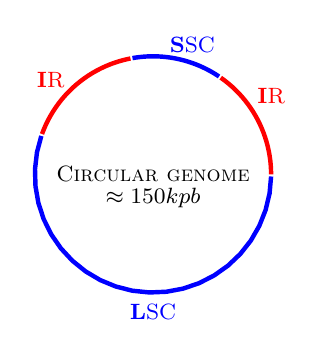
\begin{tikzpicture}
   \draw [red,ultra thick,domain=0:55] plot ({1.5*cos(\x)}, {1.5*sin(\x)});
   \draw [blue,ultra thick,domain=56:100] plot ({1.5*cos(\x)}, {1.5*sin(\x)});
   \draw [red, ultra thick, domain=101:160] plot ({1.5*cos(\x)}, {1.5*sin(\x)});
   \draw [blue, ultra thick, domain=161:359] plot ({1.5*cos(\x)}, {1.5*sin(\x)});
   \node[draw=none, fill=none] at (0,0) {\footnotesize \textsc{Circular genome }};
   \node[draw=none, fill=none] at (0,-0.3) {\footnotesize $\approx 150kpb$};
   \node[draw=none, fill=none] at (1.5,1) {\footnotesize \color{red} \textbf IR};
   \node[draw=none, fill=none] at (-1.3,1.2) {\footnotesize \color{red} \textbf IR};
   \node[draw=none, fill=none] at (0,-1.75) {\footnotesize \color{blue} \textbf LSC};
   \node[draw=none, fill=none] at (0.5,1.65) {\footnotesize \color{blue} \textbf SSC};
\end{tikzpicture}
\caption{Chloroplast genome structure}
\subcaption*{\footnotesize Inverted Repeat (IR $ \approx 23kpb$) ; Long Single Copy (LSC); Small Simple Copy (SSC $\approx 85kpb$)}
\end{figure} \\
The instances used for this study are the chloroplast genomes of the following organisms: \textit{Eucalyptus globulus, Acorus calamus, Atropa belladonna, Agrostis stolonifera, Cucumis sativus, Lecomlella madagascariensis, Oenothera elata, Pinus koraiensis} and \textit{Euglena gracilis}. Despite having the same general structure, the amount of repeated sequences is different from an instance to another, making them more or less easy to assemble.
%\vspace*{pt}
\subsection{Input data}
\begin{figure}[h!]
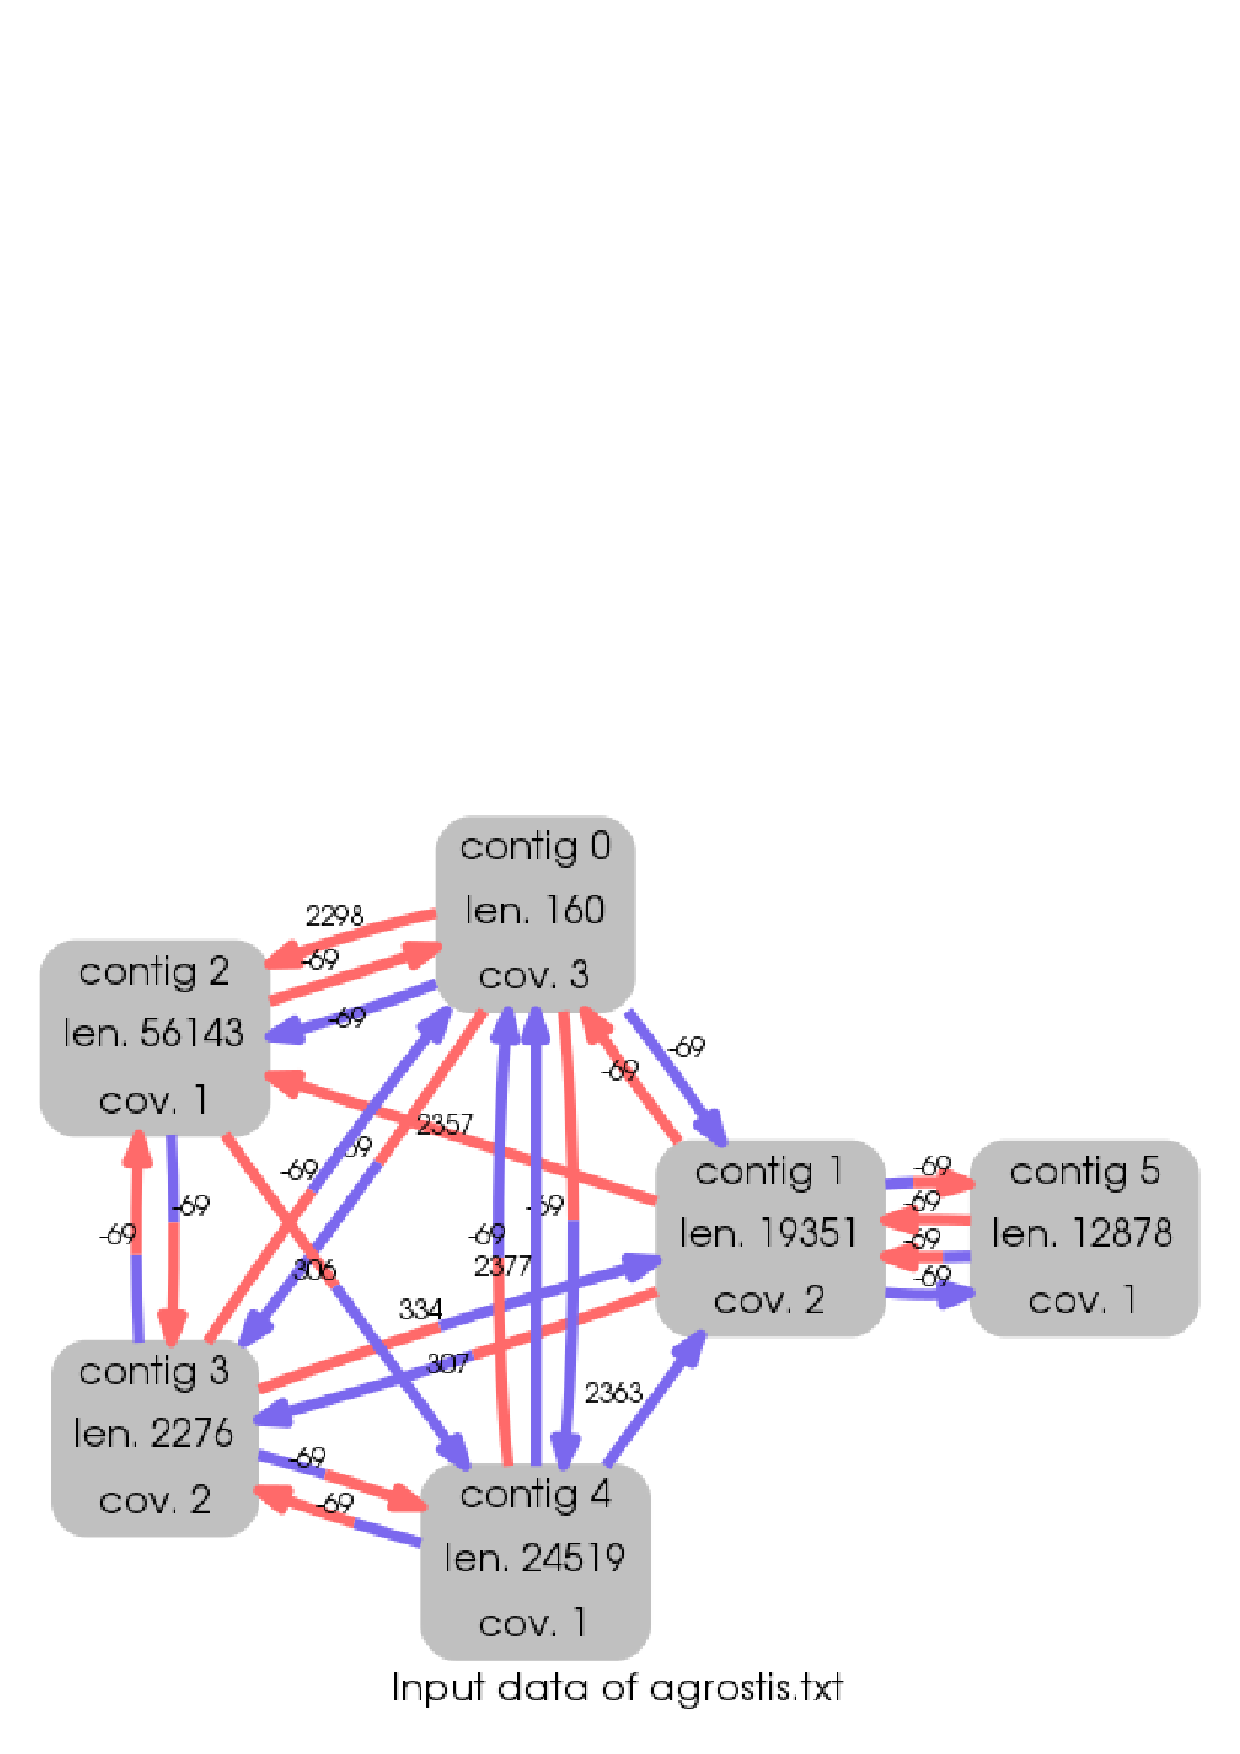
\includegraphics[scale=0.4]{agrostis_INPT}
\caption{Input data of \textit{Agrostis stolonifera} viewed in form of a graph}
\subcaption*{\footnotesize The image was generated with the \textit{graph\_generator.py} script. The color on the links indicate if the links points to the contigs in forward (blue) or reverse (red) orientation.}

\end{figure}


%-------------------------------------------------------------------------------
% BODEH!
%-------------------------------------------------------------------------------
\newpage
\section{Material and methods}
\subsection{Inspecting the input data}
\subsection{Benchmarking}
Chosen scaffolding tools to benchmark against
Benchmarking workflow
Comparisons
QUAST
Comparison function
Visualization
MUMMER
Visualization tool
%-------------------------------------------------------------------------------
% BODEH!
%-------------------------------------------------------------------------------
\section{Results}
\subsection{Data sets compared}
\subsubsection{QUAST and comparison function}
\subsubsection{Visualization}
%-------------------------------------------------------------------------------
% BODEH!
%-------------------------------------------------------------------------------
\section{Conclusion}
\clearpage
\bibliography{scaffoldingbiblio}
\bibliographystyle{naturemag}
%\printbibliography
\end{document}